\documentclass[journal]{IEEEtran}

\usepackage{cite}
\usepackage{amsmath,amssymb,amsfonts}
\usepackage[boxed]{algorithm2e}

\usepackage{graphicx}
\graphicspath{{../../Dissertacao/figuras/}}

\usepackage{textcomp}
\usepackage{xcolor}
\usepackage{booktabs}                        % AAB inserido
\usepackage[utf8]{inputenc}                  % AAB inserido
\usepackage{rotating}                        % AAB inserido
\usepackage{mathtools}                       % AAB inserido

\usepackage{bm,bbm}
\usepackage[binary-units]{siunitx}

\usepackage[caption=false,font=footnotesize]{subfig}
\DeclareMathOperator{\traco}{tr}



\begin{document}
\title{Fusion of Evidences in Intensities Channels for Edge Detection in PolSAR Images}
\author{Anderson A.\ de Borba, Maurício Marengoni, and Alejandro C.\ Frery,~\IEEEmembership{Senior Member,~IEEE}%
\thanks{A.\ A.\ de Borba is with the Dept.\ Engenharia Elétrica e Computação, Universidade Presbiteriana Mackenzie (UPM), and with IBMEC-SP, São Paulo, Brazil. anderson.borba@ibmec.edu.br}
\thanks{M.\ Marengoni is with the Dept.\ Engenharia Elétrica e Computação,
UPM, São Paulo, Brazil. mauricio.marengoni@mackenzie.br}
\thanks{A.\ C.\ Frery is with the Laboratório de Computação Científica e Análise Numérica (LaCCAN), Universidade Federal de Alagoas (UFAL), Maceió, Brazil. acfrery@laccan.ufal.br}}

\maketitle

\begin{abstract}
Polarimetric Synthetic Aperture Radar (PolSAR) sensors have reached an essential position in remote sensing. 
The images they provide have speckle noise, making their processing and analysis challenging tasks. 
We discuss an edge detection method based on the fusion of evidences obtained in the intensity channels (hh), (hv), and (vv) of PolSAR multi-look images. 
The method consists of detecting transition points in the thinnest possible range of data that covers two regions using maximum likelihood under the Wishart distribution. 
The fusion methods used are 
simple average, 
multi-resolution discrete (MR-DWT) and 
stationary (MR-SWT) wavelet transforms, 
principal component analysis (PCA), 
ROC statistics, 
and a multi-resolution method based on singular value decomposition (MR-SVD). 
A quantitative analysis suggests that MR-SWT provides the best results.
\end{abstract}

\begin{IEEEkeywords}
PolSAR, edge detection, maximum likelihood estimation, fusion methods. 
\end{IEEEkeywords}

\section{Introduction}\label{sec_01}
\IEEEPARstart{P}{olarimetric} synthetic aperture radar (PolSAR) has achieved an essential position in remote sensing. 
The data such sensors provide require specifically tailored signal processing techniques.
Among such techniques, edge detection is one of the most important operations for extracting information.
Edges are at a higher level of abstraction than mere data and, as such, provide relevant insights about the scene.

Among the available edge detection techniques for SAR and PolSAR images, it is worth mentioning:techniques based on denoising~\cite{sjx, lzly, wxbzw, law, cgaf};   
Markov random fields~\cite{bf};	
the deep learning approach~\cite{bac, ztmxzxf} applied to segmentation and classification; and
statistical techniques~\cite{gmbf, fbgm, nhfc} applied in edge detection in PolSAR and SAR imagery.


This article follows the statistical modeling approach using the techniques described in~\cite{gmbf, fbgm, nhfc} to find edge evidences, followed by fusion processes~\cite{mit, bmf_2019}. 
Our approach does not attempt to reduce the speckle, but to extract information from its statistical properties.

Instead of handling fully polarimetric data, we treat each intensity channel separately, obtain evidence of edges, and then produce a single estimator of the edge position.
With this, we quantify the contribution each channel provides to the solution of the problem.

The Gambini Algorithm~\cite{gmbf_sc} is an attractive edge detection technique.
It is local, as it finds evidence of an edge over a thin strip of data; 
it works with any model, which makes it suitable for SAR data; 
and it has shown better performance than other approaches.
This algorithm consists in casting rays, and then finding the evidence of an edge in the ray by maximizing a value function.
The value function we use is the likelihood of two samples: one inside the edge, another outside the edge.
Without loss of generality, we assume the complex scaled Wishart distribution for the fully polarimetric observations, from which Gamma laws stem for each intensity channel.
The value function depends on the estimates that index such Gamma laws; and
we estimate them by maximum likelihood.

The value function is the total likelihood.
It is non-differentiable at most points, and classical methods have difficulties in finding the maximum of a non-differentiable functions. 
We used the Generalized Simulated Annealing (GenSA)~\cite{xgsh} method to solve this problem. 

We discuss and compare six fusion methods:
Simple average~\cite{mit}, 
Multi-Resolution Discrete Wavelet, MR-DWT~\cite{n_r},
Principal Component Analysis, PCA~\cite{n_r,mit},
ROC statistics~\cite{gs},
Multi-Resolution Stationary Wavelet Transform, MR-SWT~\cite{n_r, jjly}, and 
Multi-Resolution Singular Value Decomposition, MR-SVD~\cite{naidu}.

%It aims to show the feasibility of a procedure for edge detection in PolSAR images using the fusion methods.

%The objective is to understand and quantify the importance of the information provided by each channel to improve the edge detection process.

The article is structured as follows.
Section~\ref{sec_02} describes statistical modeling.
Section~\ref{sec_03} describes edge detection for PolSAR data.
Section~\ref{sec_04} describes the approach to edge evidence fusing.
Section~\ref{sec_05} presents numerical results.
Finally, Section~\ref{sec_06} concludes the work with observations, future directions of research, and the feasibility of detecting edges in each channel of PolSAR images.

\section{Statistical modeling for PolSAR data}\label{sec_02}

Multi-looked fully polarimetric data follow the Wishart distribution with PDF defined by:
\begin{equation}
    f_{\mathbf{Z}}(\mathbf{Z};\mathbf{\Sigma},L)=\frac{L^{mL}|\mathbf{Z}|^{L-m}}{|\mathbf{\Sigma}|^{L}\Gamma_m(L)} \exp(-L\traco(\mathbf{\Sigma}^{-1}\mathbf{Z})),
    \label{eq:DistWishart}
\end{equation} 
where, $L$ is the number of looks, $\traco(\cdot)$ is the trace operator of a matrix, $\Gamma_m(L)$ is the multivariate Gamma function defined by $
	\Gamma_m(L)=\pi^{\frac{1}{2}m(m-1)} \prod_{i=0}^{m-1}\Gamma(L-i)$,
and $\Gamma(\cdot)$ is the Gamma function.
We used three $m=3$ channels in this study. 
This situation is denoted by $\mathbf{Z}\sim W(\mathbf{\Sigma}, L)$, which satisfies $E[\mathbf{Z}]=\mathbf{\Sigma}$. 
This assumption usually holds for fully developed speckle but, since we will estimate $L$ locally instead of considering the same number of looks for the whole image, we will in part take into account departures from such hypothesis.

Fully polarimetric data may be modeled by~\eqref{eq:DistWishart}.
Since we are interested in describing the information conveyed by parts of such matrix, we rely on the results presented in~\cite{hsbmp}.
In particular, we assume that the distribution of each intensity channel is a 
Gamma law with probability density function
\begin{equation}
f_Z(z;\mu,L)=\frac{L^{L}z^{L-1}}{\mu^{L}\Gamma(L)} \exp\big\{-Lz/\mu\big\},\quad z>0,
\label{func_dens_uni_gamma}
\end{equation}
where $L>0$ (rather than $L\geq1$ to allow for flexibility), and
$\mu>0$ is the mean.
The reduced log-likelihood of the sample $\bm z = (z_1,\dots,z_n)$ under this model is
\begin{equation}
\mathcal L( L,\mu; \bm z) = 
n \big[L\ln (L / \mu) - \ln \Gamma(L)\big]
+L \sum_{k=1}^{n}\ln z_k -\frac{L}{\mu}\sum_{k=1}^{n} z_k.
\label{eq:LogLikelihoodGamma}
\end{equation}

We obtain $(\widehat L, \widehat \mu)$, the maximum likelihood estimator (MLE) of $(L, \mu)$ based on $\bm z$, by maximizing~\eqref{eq:LogLikelihoodGamma} with the BFGS method~\cite{ht}.
We prefer optimization to solving $\nabla\ell=\bm 0$ for improved numerical stability.

\section{Edge Detection on a Single Data Strip}\label{sec_03}

The Gambini algorithm estimates the point at which the properties of a sample change.
It has been used with stochastic distances~\cite{nhfc}, and with the likelihood function~\cite{gmbf, fbgm} for edge detection in SAR/PolSAR imagery.
It can be adapted to any suitable measure of dissimilarity between two samples.

The algorithm starts by casting rays from a point inside the candidate region, e.g., the centroid.
Data are collected around each ray to form the sample $\bm z = (z_1,z_2,\dots,z_n)$, which is partitioned at position $j$:
$$
\bm z = (\underbrace{z_1,z_2,\dots,z_j}_{\bm z_\text{I}}, 
\underbrace{z_{j+1}, z_{j+2},\dots,z_n}_{\bm z_\text{E}}).
$$
We assume two (possibly) different models for each partition:
$\bm Z_\text{I} \sim \Gamma(\mu_\text{I},L_\text{I})$, and 
$\bm Z_\text{E} \sim \Gamma(\mu_\text{E},L_\text{E})$.
We then estimate $(\mu_\text{I},L_\text{I})$ and $(\mu_\text{E},L_\text{E})$ with $\bm z_\text{I}$ and $\bm z_\text{E}$, respectively, by maximizing~\eqref{eq:LogLikelihoodGamma}, and obtain $(\widehat{\mu}_\text{I}, \widehat{L}_\text{I})$ and $(\widehat{\mu}_\text{E}, \widehat{L}_\text{E})$.

We then compute the reduced log-likelihood of $\bm z_\text{I}$ and $\bm z_\text{E}$:
\begin{equation}\label{eq:TotalLogLikelihood}
\begin{aligned}
%\ell(j&;\bm z_\text{I},\bm z_\text{E}) = \\
\mathcal L(j&;\widehat{\mu}_I, \widehat{L}_I,\widehat{\mu}_E, \widehat{L}_E)=\\
&j \big[\widehat{L}_\text{I}\ln (\widehat{L}_\text{I} / \widehat{\mu}_\text{I}) - \ln \Gamma(\widehat{L}_\text{I})\big]
+\widehat{L}_\text{I} \sum_{k=1}^{j}\ln z_k -\frac{\widehat{L}_\text{I}}{\widehat{\mu}_\text{I}}\sum_{k=1}^{j} z_k +\\
&(n-j) \big[\widehat{L}_\text{E}\ln (\widehat{L}_\text{E} / \widehat{\mu}_\text{E}) - \ln \Gamma(\widehat{L}_\text{E})\big]
+\widehat{L}_\text{E} \sum_{k=j+1}^{n}\ln z_k -\\ &\frac{\widehat{L}_\text{E}}{\widehat{\mu}_\text{E}}\sum_{k=j+1}^{n} z_k,
\raisetag{2.2em}
\end{aligned}
\end{equation}
and the estimate of the edge position on the ray is the coordinate $\widehat\jmath$ which maximizes it.

Algorithm~\ref{Algo:GambiniEdgeDetection} is the pseudocode of the basic edge detection with the Gambini Algorithm.
We found that one hundred rays is a good compromise between spatial continuity and computational load.
Also, $\min_s$ is the minimum sample size that we set to $14$.

\begin{algorithm}[hbt]
\SetAlgoLined
\KwData{$n_c$ intensity bands, centroid, number of rays}
\KwResult{$n_c$ binary images with evidences of edges}
%initialization\;
\For{each band $1\leq c\leq n_c$}{
	\For{each ray passing through the centroid}{
		$\bm z = (z_1,z_2,\dots,z_n)\leftarrow$ data collected around the ray with the Bresenham's midpoint line algorithm\;
		\For{each $\min_s\leq j\leq n-\min_s$}{\nllabel{Line:InitFor}
			Partition the sample as $\bm z_{\text{I}}=(z_{\min_s},\dots,z_j)$ and 
			$\bm z_{\text{E}}=(z_{j+1},\dots,z_{n-\min_s})$\;
			Compute $(\widehat{\mu}_\text{I}, \widehat{L}_\text{I})$ with $\bm z_{\text{I}}$, and $(\widehat{\mu}_\text{E}, \widehat{L}_\text{E})$ with $\bm z_{\text{E}}$\;
			Compute the total log-likelihood at $j$ as $\mathcal L(j;\widehat{\mu}_I, \widehat{L}_I,\widehat{\mu}_E, \widehat{L}_E)$\;
		}
		$\widehat\jmath\leftarrow$ the value of $j$ at which the log-likelihood function is maximized\;
		\Return $(\widehat x, \widehat y)$, the coordinates of each $\widehat\jmath$\;
	}
\Return the binary image $\widehat{\bm\jmath}_c$ with $1$ at every $(\widehat x, \widehat y)$, and $0$ otherwise.
}
\caption{Gambini algorithm for intensity channels}\label{Algo:GambiniEdgeDetection}
\end{algorithm}

In our implementation, we replace the exhaustive sequential search (the innermost \textbf{for} loop) by Generalized Simulated Annealing (GenSA~\cite{xgsh}).

%Notice that this approach can be extended and/or modified to cope with any kind of data.
%We will see ways of fusing these evidences in the next section.

\section{Fusion of Evidences}\label{sec_04}

Assume we have $n_c$ binary images $\{\widehat{\bm\jmath}_c\}_{1\leq c\leq n_c}$ in which~$1$ denotes an estimate of edge and $0$ otherwise.
They have common size $m\times n$; denote $\ell=mn$.
These images will be fused to obtain the binary image $\bm I_F$.

%Denote in the following $\widehat{\bm\jmath}_c$ the binary image with same support as the input data $c$ ($m$ lines and $n$ columns; denote $\ell=mn$), where $1$ denotes an estimate of edge and $0$ otherwise.
%We have $n_c$ of these image to fuse, and the result of the fusion will be denoted $\bm I_F$.

We compare the results of six fusion techniques, namely:
simple average, 
multi-resolution discrete wavelet transform (MR-DWT),
principal components analysis (PCA), 
ROC statistics,
multi-resolution stationary wavelet transform (MR-SWT), and
multi-resolution singular value decomposition (MR-SVD).

%The estimated evidence image and the fusion image are defined to perform the fusion techniques. The first can be defined as $\widehat\jmath_c(x,y)$, where $x$ and $y$, indicate the range of pixels in an image equal in size to the data image chosen for analysis. The image is binary, where the value one is put on the pixel estimated as edge evidence by the MLE method, and zero on the other pixels, for each channel. The second called $\text{I}_F(x,y)$ is the result of the fusion method. 

%Refs.~\cite{bmf_2019,n_r,mit,gs,fawcett} provide details about the three first.
%We describe the two latter below.

\subsection{Simple Average}
The simple average fusion method proposes the arithmetic mean of the edge evidence in each of the $n_c$ channels:
$\bm I_F(x,y)=(n_c)^{-1}\sum_{c=1}^{n_c} \widehat{\bm\jmath}_c(x,y)$,
where $1\leq x\leq m$ indexes the rows, and $1\leq y\leq n$ the columns of the image.
%where $\widehat\jmath_c$ denotes the estimate obtained in channel $c$.

\subsection{Multi-Resolution Discrete Wavelet -- MR-DWT} 
This section is based on~\cite{n_r}.
%We apply DWT filters separately in the vertical and horizontal directions of each image $\bm{\widehat\jmath}_c$, then down-sampled by a factor of two. 
%In this way, each image is filtered by the low pass filter $\text{L}$ in the vertical direction and the high pass filter $\text{H}$ in the horizontal direction, then down-sampled to create the matrices coefficients  $\bm{\widehat\jmath}_{c\text{L}}$ and $\bm{\widehat\jmath}_{c\text{H}}$.
We apply DWT filters on each binary image $\bm{\widehat\jmath}_c$: a low-pass filter $\bm L$ in the vertical direction, and a high-pass filter $\bm H$ in the horizontal direction, then both are down-sampled to create the coefficient matrices $\bm{\widehat\jmath}_{c\text{L}}$ and $\bm{\widehat\jmath}_{c\text{H}}$.
These operations are repeated on the coefficient matrices, leading to $\bm{\widehat\jmath}_{c\text{LL}}$, $\bm{\widehat\jmath}_{c\text{LH}}$, $\bm{\widehat\jmath}_{c\text{HL}}$, and $\bm{\widehat\jmath}_{c\text{HH}}$.

%%% ACF Detalhar as operações usando a notação acima: a média é pixel-a-pixel? quais bandas são promediadas?
%%% AAB A média é pixel a pixel. Todas as bandas são usadas na média. Vou tentar deixar claro no texto. Creio que respondi no item 2 abaixo.
%%% AAB Eu entendo que investigar outros tipo de ponderação (suprimir canais, por exemplo) pode ser realizado. Ainda não consegui fazer esses testes.
%%% AAB O nivel de resolução que uso é 1, esse é outro ponto de investigação, seria interessante aumentar esse nível e ver o que acontece na fusão. Tb não consegui realizar esses teste. Inseri no item 1) abaixo a info sobre o nível de resolução.
The DWT fusion method has the following steps:
\begin{enumerate}
\item Calculate the DWT decomposition $\bm{\widehat\jmath}_{c\text{LL}}$, $\bm{\widehat\jmath}_{c\text{LH}}$, $\bm{\widehat\jmath}_{c\text{HL}}$, and $\bm{\widehat\jmath}_{c\text{HH}}$, for each channel.
\item Compute $\bm{\bar\jmath}_{c\text{HH}}$, the pixel-wise mean of all $\bm{\widehat\jmath}_{c\text{HH}}$ decompositions.
\item Find the pixel-wise maximum of $\bm{\widehat\jmath}_{c\text{LL}}$, $\bm{\widehat\jmath}_{c\text{LH}}$, $\bm{\widehat\jmath}_{c\text{HL}}$: $\bm{\bar\jmath}_{c\text{LL}}$, $\bm{\bar\jmath}_{c\text{LH}}$, and $\bm{\bar\jmath}_{c\text{HL}}$.
%%% AAB(03/03/2020) tenho uma dúvida, o máximo(pixel a pixel) deve ser calculada entre os operadores da decomposiçcao em cada canal. Não seria bom deixar claro como no item anterior?
\item The result of the fusion $I_F$ is the inverse DWT transform of the coefficient matrices $\bm{\bar\jmath}_{c\text{HH}}$, $\bm{\bar\jmath}_{c\text{LL}}$, $\bm{\bar\jmath}_{c\text{LH}}$, and $\bm{\bar\jmath}_{c\text{HL}}$.
\end{enumerate}
%%% ACF Aqui dizer que é a Inverse DWT do que
\subsection{Principal Component Analysis -- PCA}

%%% ACF Revisar e corrigir a notação; usar notação matemática sempre que necessário
This section is based on~\cite{n_r,mit}.
The method is comprised of the following steps:
\begin{enumerate}
\item Stack the binary images $\bm{\widehat\jmath}_c$ in column vectors to obtain the matrix $\bm X_{\ell\times n_c}$.
%\item Calculate the average of the elements of these columns, generating a vector of dimension of $1\times nc$.
%%% ACF A matriz de covariância é invariante a traslações. Precisa deste passo?
%\item subtract the average of each column from $\text Y$, resulting in a matrix of the same dimension of $\text X$; 
\item Calculate the covariance matrix $\bm C_{n_c\times n_c}$ of $\bm X_{\ell\times n_c}$.
\item Compute the matrices of eigenvalues ($\bm\Lambda$) and eigenvectors ($\bm V$) of the covariance matrix, sorted in decreasing order by the eigenvalues. %The matrices generated by the eigenvalues, on the principal diagonal, and the eigenvectors placed in columns;
%%% ACF O que é V_c?
\item Compute the vector $\bm P=(\sum_{c=1}^{n_c} V(c))^{-1}{\bm V}$, where $\bm V$ is eigenvector associated with the highest eigenvalue of $\bm C_{n_c\times n_c}$; notice that $\sum_{c=1}^{n_c} P(c)=1$.
\item Fuse $\bm I_F(x,y)=\sum_{c=1}^{n_c} P(c)\bm{\widehat\jmath}_c(x,y)$.
\end{enumerate}

\subsection{ROC Statistics}
The ROC method was proposed and described on~\cite{gs}:
\begin{enumerate}
%\item the evidence of edges in each channels $\bm{\widehat\jmath}_c$, with $c=1,\dots,nc$ in a binary way;
%%% AAB(03/03/2020) Aqui fico em dúvida se coloco "matrices" ou  "binary images".  
\item Add the binary images $\bm{\widehat\jmath}_c$ to produce the frequency matrix ($\bm V$).
\item Use thresholds ranging from $t=1,\dots,n_c$ on $\bm V$ to generate matrices $\bm M_t$.
\item Compare each $\bm M_t$ with all $\bm{\widehat\jmath}_c$, find the confusion matrix to generate the ROC curve. 
The optimal threshold corresponds to the point of the ROC curve closest (in the sense of the Euclidean distance) to the diagnostic line.
\item The fusion $\bm I_F$ is the matrix $\bm M_t$ which corresponds to the optimal threshold.
\end{enumerate}

\subsection{Multi-Resolution Stationary Wavelet Transform -- MR-SWT}  
This section is based on~\cite{n_r, jjly}. The difference between MR-DWT and MR-SWT method is the replacement of the method discrete wavelet transform (DWT) by the method stationary wavelet transform SWT. 
%%% ACF Esclarecer quais são estes filtros

\subsection{Multi-Resolution Singular Value Decomposition -- MR-SVD}

MR-SVD Fusion~\cite{naidu} works similarly to MR-DWT. 
The difference consists in changing the DWT filters by the SVD filters. 
The MR-SVD fusion method can be summarized as follows:
\begin{enumerate}
%\item Organize the binary image $\bm{\widehat\jmath}_c$ in matrices $\text{X}_\ell$ with dimension $4\times\frac{\text{M}}{2}\frac{\text{N}}{2}$ according to~\cite{naidu}, where M is the number of rows and N is the number of columns in $\bm{\widehat\jmath}_c$, and $\ell$ is the level resolution to set. In this work is used one resolution level;
\item Organize the binary image $\bm{\widehat\jmath}_c$ as non-overlapping $2\times 2$ blocks, and arrange each block as a $4\times 1$ vector by stacking columns to form the data matrix $\bm X_1$ with dimension ${4\times{\ell}/{4}}$.
%, where M is the number of rows and N is the number of columns in $\bm{\widehat\jmath}_c$, 
%and $\ell$ is the level resolution to set. In this work is used one resolution level.
%%% ACF Repare que não usou M nem N
%\item Find the SVD decomposition
% of $\bm X_1=\bm U_1 \bm S_1 \bm V_1^T$, where $\bm U_1$ and $\bm V_1$ are  unitary and they have dimensions ${4\times 4}$ e ${\ell}/{4}\times{\ell}/{4}$ respectively. The diagonal entries $S_{ii}$ of $\bm S_1$ are known as the singular values of $\bm X_1$ and it have dimension $4\times{\ell}/{4}$. The singular values are sorted in descending, and they are putting in the diagonal principal of the matrix, other entries must be zeros. 
\item Find the SVD decomposition of $\bm X_1=\bm U_1 \bm S_1 \bm V_1^T$, where $\bm U_1$ is a ${4\times 4}$ unitary matrix, $\bm S_1$ is a rectangular diagonal matrix $4\times{\ell}/{4}$ known as singular values matrix, and $\bm V_1$ is a ${\ell}/{4}\times{\ell}/{4}$~unitary matrix. The singular values are ordered in a decreasing order.
% and calculate $\bm T_1=\bm X_1 \bm X_1^T=\bm U_1 \bm S_1^2 \bm U_1^T\Sigma \bm V^T$, where $s(1)\geq s(2) \geq s(3) \geq s(4)$ comprise the singular value matrix $\bm S_1$, 
%%% ACF Não definiu nem usou s(1), s(2) etc
%%% AAB Os s(1), s(2), s(3) e s(4) são usados para gerar a matriz $S$
% and $\bm U_1$ is unitary.
\item 
Transform the lines of $\widehat{\bm X}_1=\bm U_1^T\bm X_1=\bm S_1 \bm V_1^T$ into new matrices with dimensions ${m}/{2}\times{n}/{2}$: $\{\bm\Phi_1, \bm\Psi_{1\text{V}}, \bm\Psi_{1\text{H}}, \bm\Psi_{1\text{D}}\}$. 
%\item Repeat the procedure on $\Phi_r$ $R$ times. Where $r=1,\dots,\text{R}$ and, R is lowest resolution index. 
\item Repeat the procedure (1) on $\bm\Phi_r$ by $r=2$ up to the lowest resolution level $R$. 
\item The MR-SVD decomposition in each channel is
\begin{equation}\nonumber
\widehat{\bm X}_c\rightarrow \left\{\bm \Phi_\text{R}^c,\{\bm\Psi_{r\text{V}}^c,\bm\Psi_{r\text{H}}^c,\bm\Psi_{r\text{D}}^c \}_{r=1}^\text{R},\{\bm U_r^c	\}_{r=1}^\text{R} \right\}.
\end{equation}
%\item Once the SVD is applied to level $\ell$ the fusion process is executed as follow: In the operators $\Psi_\ell^\text{V}$, $\Psi_\ell^\text{H}$ and $\Psi_\ell^\text{D}$, the maximum is found among all channel, pixel by pixel, resulting in new operators $\bar{\Psi}_\ell^\text{V}$, $\bar{\Psi}_\ell^\text{H}$ and $\bar{\Psi}_\ell^\text{D}$. 
%The operators $\Phi_L$, and $\text{U}_\ell$ are averaged over all the channels, pixel by pixel.
\item Once the decomposition is applied to all channels, 
compute the average of $\bm\Phi_R^c$ ($\bm\Phi_\text{R}^f$) in the lowest resolution level, and the average 
of $\bm U_r^c$ ($\bm U_\text{r}^f$), for each $r$, where $f$ denotes the fusion among channels. 
%\item Find the pixel-wise maxima of $\bm\Psi_r^\text{V}$, $\bm\Psi_r^\text{H}$ and $\bm\Psi_r^\text{D}$ :$ \prescript{}{2}{\mathbf{\bm\Psi}}^{V}_{r}$ $\overline{\bm\Psi}_r^\text{V}$, $\overline{\bm\Psi}_r^\text{H}$ and $\overline{\bm\Psi}_r^\text{D}$.
\item Find the pixel-wise maxima of $\bm\Psi_{r\text{V}}^c$, $\bm\Psi_{r\text{H}}^c$ and $\bm\Psi_{r\text{D}}^c$: $ \bm\Psi_{rV}^f$ $\bm\Psi_{r\text{V}}^f$, $\bm\Psi_{r\text{H}}^f$ and $\bm\Psi_{r\text{D}}^f$.
\item The fusion $\bm I_F$ is the SVD transformation for each level $r=\text{R},\dots,1$,  
\begin{equation}\nonumber
\bm I_F\leftarrow \left\{\bm \Phi_\text{R}^f,\{\bm\Psi_{r\text{V}}^f,\bm\Psi_{r\text{H}}^f,\bm\Psi_{r\text{D}}^f \}_{r=\text{R}}^1,\{\bm U_r^f\}_{r=\text{R}}^1 \right\}.
\end{equation}
\end{enumerate}

\section{Results}\label{sec_05}

\subsection{PolSAR image}

We used a $750\times 1024$ pixels AIRSAR PolSAR image of Flevoland, L-band, for the tests. 
Fig.~\ref{roi_gt}\subref{flevoland_radial_4look} shows the ROI, with the radial lines where edges are detected. 
Fig.~\ref{roi_gt}\subref{gt_flevoland} shows the ground reference in red.  

\begin{figure}[hbt]
   \centering
     \subfloat[Image, Region of Interest (ROI), and rays. \label{flevoland_radial_4look}]{%  
       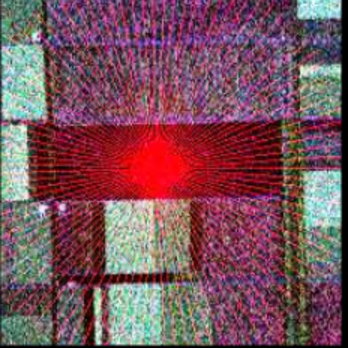
\includegraphics[width=0.229\textwidth]{flevoland_radial_4_look_black_crop}}
     \subfloat[Ground reference\label{gt_flevoland}]{%
       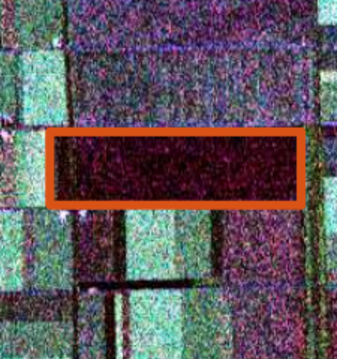
\includegraphics[width=0.216\textwidth]{gt_flevoland_crop}
     }
    \caption{Flevoland image in Pauli decomposition, and ground reference}
    \label{roi_gt}
\end{figure}

Figs.~\ref{evidencias_hh_hv_vv}\subref{evidencias_hh_hv_vv:a}, \ref{evidencias_hh_hv_vv}\subref{evidencias_hh_hv_vv:b}, and~\ref{evidencias_hh_hv_vv}\subref{evidencias_hh_hv_vv:c} show, respectively, the edge evidences in the $\text{hh}$, $\text{hv}$ and $\text{vv}$ channels as obtained by MLE.

It is worth noting that GenSA has accurately identified the maximum value of $\ell$ (Eq.~\eqref{eq:TotalLogLikelihood}), even in the presence of multiple local maxima. 
A visual assessment leads to conclude that the best results are provided by $\text{hv}$, although with a few points far from the actual edge.

   \begin{figure}[hbt]
	\centering
     \subfloat[Channel $\text{hh}$ \label{evidencias_hh_hv_vv:a}]{%
       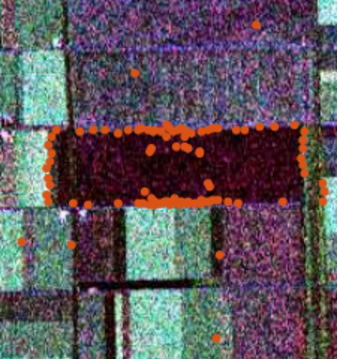
\includegraphics[width=0.32\linewidth]{flevoland_hh_evid_param_L_mu_14_pixel_crop}
     }
     \subfloat[Channel $\text{hv}$ \label{evidencias_hh_hv_vv:b}]{%
       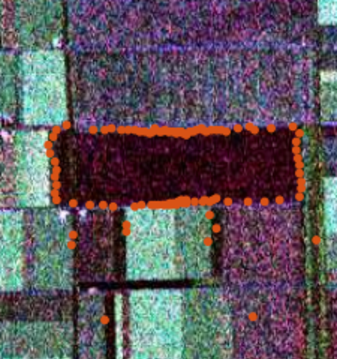
\includegraphics[width=0.32\linewidth]{flevoland_hv_evid_param_L_mu_14_pixel_crop}
     }
     \subfloat[Channel $\text{vv}$ \label{evidencias_hh_hv_vv:c}]{%
       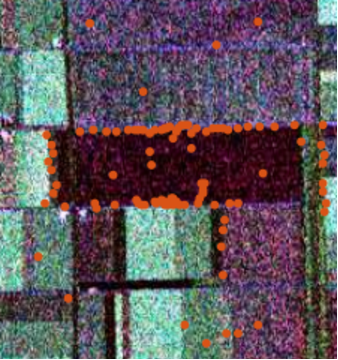
\includegraphics[width=0.32\linewidth]{flevoland_vv_evid_param_L_mu_14_pixel_crop}
     }
     \caption{Edges evidences from the three intensity channels}
     \label{evidencias_hh_hv_vv} 
   \end{figure}

Figs.~\ref{fusion_met}\subref{fusion_met:a}, \subref{fusion_met:b}, \subref{fusion_met:c}, \subref{fusion_met:d}, \subref{fusion_met:e}, and~\subref{fusion_met:f} show the results of fusing these evidences. 

%%% AAB inserido 
% Figura da região 2 com 80 pixel para as radiais 1 até 64 e 60 pixel para as radiais 65 até 100.
   \begin{figure}[hbt]
	\centering
     \subfloat[Channel $\text{hh}$ \label{evidencias_r2_hh_hv_vv:a}]{%
       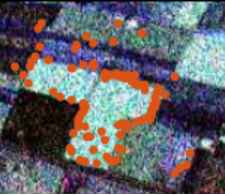
\includegraphics[width=0.32\linewidth]{flev_r2_hh_evid_L_mu_14_80_60strip_pixel_crop}
     }
     \subfloat[Channel $\text{hv}$ \label{evidencias_r2_hh_hv_vv:b}]{%
       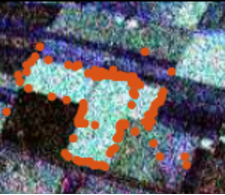
\includegraphics[width=0.32\linewidth]{flev_r2_hv_evid_L_mu_14_80_60strip_pixel_crop}
     }
     \subfloat[Channel $\text{vv}$ \label{evidencias_r2_hh_hv_vv:c}]{%
       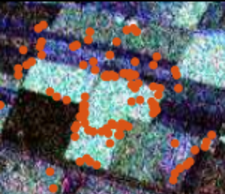
\includegraphics[width=0.32\linewidth]{flev_r2_vv_evid_L_mu_14_80_60strip_pixel_crop}
     }
     \caption{Edges evidences from the three intensity channels to ROI II - cuidado}
     \label{evidencias_r2_hh_hv_vv} 
   \end{figure}

%%% AAB inserido 
% Figura da região 2 com 60 pixel para todas radiais menos na faixa de radiais 51 até 64 (80 pixel).
   \begin{figure}[hbt]
	\centering
     \subfloat[Channel $\text{hh}$ \label{evidencias_r2_hh_hv_vv:a}]{%
       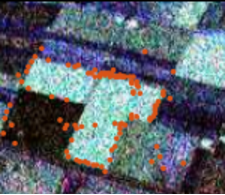
\includegraphics[width=0.32\linewidth]{flev_r2_hh_evid_L_mu_14_60_80strip_pixel_crop}
     }
     \subfloat[Channel $\text{hv}$ \label{evidencias_r2_hh_hv_vv:b}]{%
       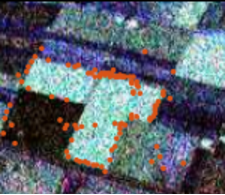
\includegraphics[width=0.32\linewidth]{flev_r2_hv_evid_L_mu_14_60_80strip_pixel_crop}
     }
     \subfloat[Channel $\text{vv}$ \label{evidencias_r2_hh_hv_vv:c}]{%
       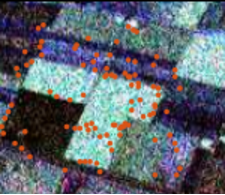
\includegraphics[width=0.32\linewidth]{flev_r2_vv_evid_L_mu_14_60_80strip_pixel_crop}
     }
     \caption{Edges evidences from the three intensity channels to ROI II - cuidado 2}
     \label{evidencias_r2_hh_hv_vv} 
   \end{figure}

%%% AAB inserido 
% Figura da região san francisco
% tamanho da radial 40
% folga nas extremidades das radiais 8 pixels
   \begin{figure}[hbt]
	\centering
     \subfloat[Channel $\text{hh}$ \label{evidencias_sf_hh_hv_vv:a}]{%
       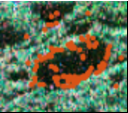
\includegraphics[width=0.32\linewidth]{sf_hh_evid_param_L_mu_8_pixel_crop}
     }
     \subfloat[Channel $\text{hv}$ \label{evidencias_sf_hh_hv_vv:b}]{%
       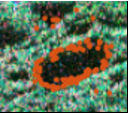
\includegraphics[width=0.32\linewidth]{sf_hv_evid_param_L_mu_8_pixel_crop}
     }
     \subfloat[Channel $\text{vv}$ \label{evidencias_sf_hh_hv_vv:c}]{%
       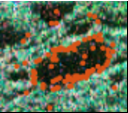
\includegraphics[width=0.32\linewidth]{sf_vv_evid_param_L_mu_8_pixel_crop}
     }
     \caption{Edges evidences from the three intensity channels to San Francisco}
     \label{evidencias_sf_hh_hv_vv} 
   \end{figure}


%Thus, one can see that the time for the PCA method is 2.19 times longer than the simple average.  

The simple average and PCA produce similar results.
MR-SVD produces considerably less outliers than the other methods, at the cost of longer processing time.
ROC produces accurate edges, with few outliers, but sparsely. 
%One way to get around this problem would be to increase the number of channels considered using other PDF.
Both wavelet-based methods (DWT and SWT) produce too dense edges and many outliers.

%The post-processing is an option to be used in all the fusion methods. 
%An idea can be found in Ref.~\cite{fbgm}. 


\begin{figure}[hbt]
	\centering
     \subfloat[Average fusion\label{fusion_met:a}]{%
       %\includegraphics[width=0.2\textwidth]{example-image-a}
       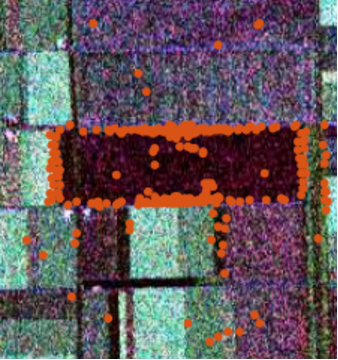
\includegraphics[width=0.48\linewidth]{flevoland_fus_media_param_L_mu_14_pixel_crop}
     }
     \subfloat[DWT fusion\label{fusion_met:b}]{%
       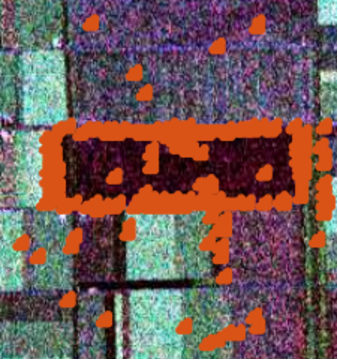
\includegraphics[width=0.48\linewidth]{flevoland_fus_dwt_param_L_mu_14_pixel_crop}
     }\\
     \subfloat[PCA fusion \label{fusion_met:c}]{%
       %\includegraphics[width=0.2\textwidth]{example-image-a}
       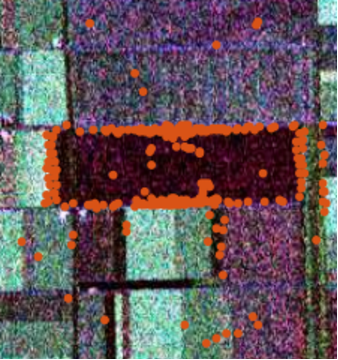
\includegraphics[width=0.48\linewidth]{flevoland_fus_pca_param_L_mu_14_pixel_crop}       
     }
     \subfloat[ROC fusion\label{fusion_met:d}]{%
       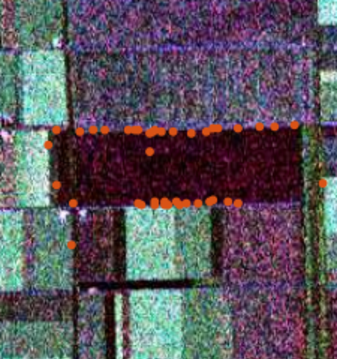
\includegraphics[width=0.48\linewidth]{flevoland_fus_roc_param_L_mu_14_pixel_crop}
     }\\
     \subfloat[MR-SWT fusion\label{fusion_met:e}]{%
       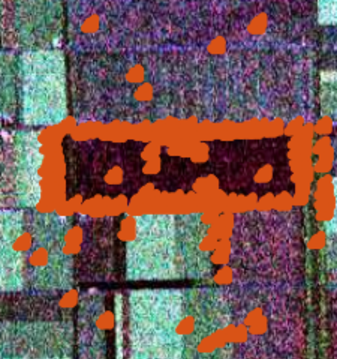
\includegraphics[width=0.48\linewidth]{flevoland_fus_swt_param_L_mu_14_pixel_crop}
     }
     \subfloat[MR-SVD fusion\label{fusion_met:f}]{%
       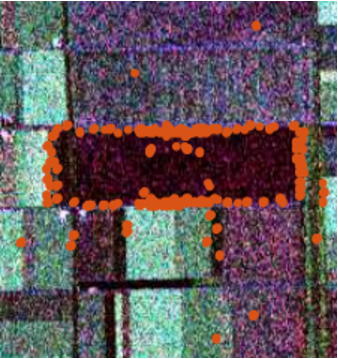
\includegraphics[width=0.48\linewidth]{flevoland_fus_svd_param_L_mu_14_pixel_crop}
     }
     \caption{Results of applying the six fusion methods}
     \label{fusion_met}
\end{figure}

%%% AAB inserido 
% Figura para a fusão da região 2 com 80 pixel para as radiais 1 até 64 e 60 pixel para as radiais 65 até 100.

\begin{figure}[hbt]
	\centering
     \subfloat[Average fusion\label{fusion_r2_met:a}]{%
       %\includegraphics[width=0.2\textwidth]{example-image-a}
       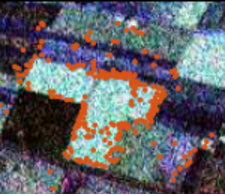
\includegraphics[width=0.48\linewidth]{flev_r2_media_L_mu_14_80_60strip_pixel_crop}
     }
     \subfloat[DWT fusion\label{fusion_r2_met:b}]{%
       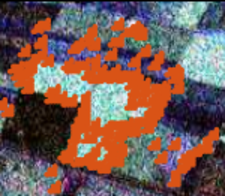
\includegraphics[width=0.48\linewidth]{flev_r2_dwt_L_mu_14_80_60strip_pixel_crop}
     }\\
     \subfloat[PCA fusion \label{fusion_r2_met:c}]{%
       %\includegraphics[width=0.2\textwidth]{example-image-a}
       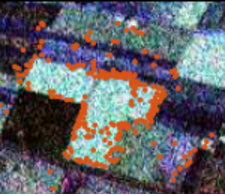
\includegraphics[width=0.48\linewidth]{flev_r2_pca_L_mu_14_80_60strip_pixel_crop}       
     }
     \subfloat[ROC fusion\label{fusion_r2_met:d}]{%
       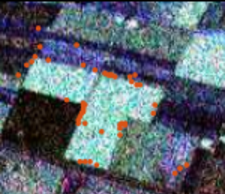
\includegraphics[width=0.48\linewidth]{flev_r2_roc_L_mu_14_80_60strip_pixel_crop}
     }\\
     \subfloat[MR-SWT fusion\label{fusion_r2_met:e}]{%
       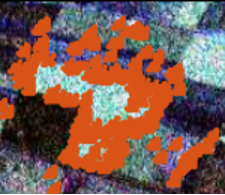
\includegraphics[width=0.48\linewidth]{flev_r2_swt_L_mu_14_80_60strip_pixel_crop}
     }
     \subfloat[MR-SVD fusion\label{fusion_r2_met:f}]{%
       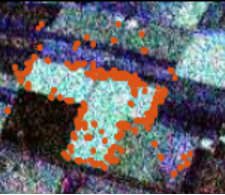
\includegraphics[width=0.48\linewidth]{flev_r2_svd_L_mu_14_80_60strip_pixel_crop}
     }
     \caption{Results of applying the six fusion methods to ROI II}
     \label{fusion_r2_met}
\end{figure}



%%%% sf 40 pixel
\begin{figure}[hbt]
	\centering
     \subfloat[Average fusion\label{fusion_sf_met:a}]{%
       %\includegraphics[width=0.2\textwidth]{example-image-a}
       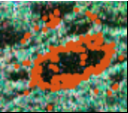
\includegraphics[width=0.48\linewidth]{sf_fus_media_param_L_mu_8_pixel_crop}
     }
     \subfloat[DWT fusion\label{fusion_sf_met:b}]{%
       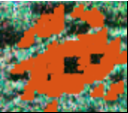
\includegraphics[width=0.48\linewidth]{sf_fus_dwt_param_L_mu_8_pixel_crop}
     }\\
     \subfloat[PCA fusion \label{fusion_sf_met:c}]{%
       %\includegraphics[width=0.2\textwidth]{example-image-a}
       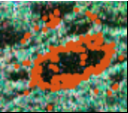
\includegraphics[width=0.48\linewidth]{sf_fus_pca_param_L_mu_8_pixel_crop}       
     }
     \subfloat[ROC fusion\label{fusion_sf_met:d}]{%
       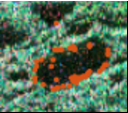
\includegraphics[width=0.48\linewidth]{sf_fus_roc_param_L_mu_8_pixel_crop}
     }\\
     \subfloat[MR-SWT fusion\label{fusion_sf_met:e}]{%
       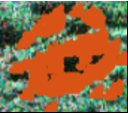
\includegraphics[width=0.48\linewidth]{sf_fus_swt_param_L_mu_8_pixel_crop}
     }
     \subfloat[MR-SVD fusion\label{fusion_sf_met:f}]{%
       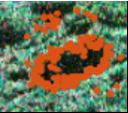
\includegraphics[width=0.48\linewidth]{sf_fus_svd_param_L_mu_8_pixel_crop}
     }
     \caption{Results of applying the six fusion methods to San Francisco}
     \label{fusion_sf_met}
\end{figure}





Figure~\ref{probability_edge_detc} shows the error of $\widehat\jmath$ in finding the true edge, as measured on $100$ radial lines: the minimum Euclidean distance among the ground truth pixel and the several pixels detected in the fusion methods.
We use relative frequencies to estimate the probability of having an error smaller than a number of pixels. 
Denoting $H(k)$ the number of replications for which the error is less than $k$ pixels, an estimate of this probability is $f(k)={H(k)}/{n_r}$, where $n_r$ is number of radii. 
In our analysis, $k$ varies between $1$ and $10$, and $n_r=100$. 
The algorithm is described in Ref.~\cite{fbgm}.

\begin{figure}[hbt]
\centering
	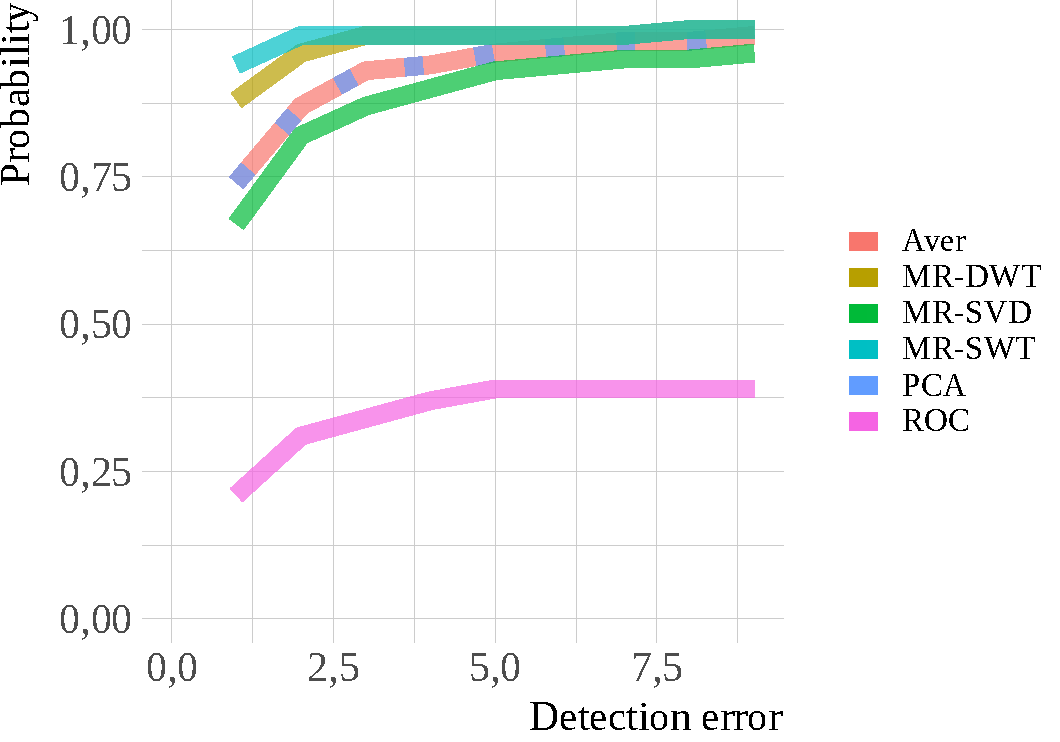
\includegraphics[width=.8\linewidth]{metricas_6_fusao_flevoland}
	\caption{Probability of detecting in fusion methods.}
\label{probability_edge_detc}
\end{figure}

\subsection{Implementation Details}

The system presented here was executed on a Intel\copyright\ Core i7-9750HQ CPU \SI{2.6}{\giga\hertz} \SI{16}{\giga\byte} RAM computer.  
The method for detecting edge evidence MLE was implemented in the R language.
The fusion methods were implemented in Matlab. 

Table~\ref{metrica_de_tempo} shows the running times (absolute and relative to the fastest method).

\begin{table}[hbt]
	\centering
	\caption{Processing times (fusion method).}\label{metrica_de_tempo}
	\begin{tabular}{@{}lrrrrrr@{}} \toprule
		Method       & Aver   &   PCA      &  MR-DWT  & MR-SWT &  ROC  &  MR-SVD \\ \midrule
		Time (s)      & 0.01      & 0.02       &  0.08 & 0.18      &  0.40       & 1.11  \\
		Rel. time     & 1.00      & 2.19       &  9.25 & 21.05     &  46.59      & 129.57  \\ \bottomrule
	\end{tabular}
\end{table}

\section{Conclusion}\label{sec_06}

We found evidence of edges using the maximum likelihood method under the Wishart model for PolSAR data. 
The evidence was found in each of the three intensity channels of an AIRSAR L-band image over Flevoland.

The best edge evidence was observed on the hv channel. We assessed the result by checking the closeness of the fused points to the actual edge, by the presence of outliers, and by the blurring effect.

We applied simple average, MR-DWT, PCA, ROC, MR-SWT, and MR-SVD fusion methods to aggregate the evidence obtained in the three channels.
The best result was produced by the Multi-Resolution Stationary Wavelet Transform (MR-SWT) with a moderate cost of the processing time.
%We assessed the results by checking the closeness of the fused points to the actual edge, by the presence of outliers, and by the blurring effect.

We highlight two avenues for future improvement of the fusion:
\begin{enumerate}
	\item increasing the number of evidences.
	This is possible, since fully polarimetric data are richer than mere intensity channels; and
	\item post-processing of both partial evidences and fusion.
\end{enumerate}

%The aims to show the feasibility of a procedure for edge detection in PolSAR images using the fusion methods was reach. 
\bibliographystyle{IEEEtran}
\bibliography{RefsTengars2020}
\end{document}

